\section{Zapewnienie spójności danych}

\begin{frame}{Spójność danych}
	
	\begin{alertblock}{Spójność/integralność danych}
		Możliwość stwierdzenia, że dane nie zostały nieautoryzowanie zmienione, dodane, usunięte.
	\end{alertblock}

	\begin{itemize}
		\item Szalenie ważne jest, abyśmy mogli stwierdzić z \emph{dużą dozą pewności}, iż dane po stronie odbiorcy i nadawcy są dokładnie takie same.
		
		\item Chcielibyśmy móc to sprawdzić, przesyłając znacząco mniej danych niż same dane.
		
		\item Do tego celu fenomenalnie nadają się kryptograficzne funkcje hashujące.
		
	\end{itemize}	

\end{frame}

\begin{frame}{Kryptograficzne funkcje haszujące}
	
	Kryptograficzna funkcja haszująca dla danych bajtów wejściowych zwraca stosunkowo dużą liczbę, typowo 128--512 bitów.
	
	Musi mieć tę własność, że najdrobniejsza zmiana danych wejściowych --- np. flipnięcie 1 bitu wśród 100 GiB --- całkowicie zmienia wyjście tej funkcji.
	
	Równie ważna własność --- dla danej wartości funkcji jest niesłychanie trudno spreparować generujące ją wejście.
	
	Teraz: jeśli odbiorca i nadawca porównają kryptograficzny skrót ze swych kopii danych, i jeśli skróty te będą takie same, z dość dużym prawdopodobieństwem dane są identyczne.
	
\end{frame}

\begin{frame}{Prawdopodobieństwo kolizji dla 128-bitowej funkcji}
	
	W poprzednim slajdzie mówimy o dużym prawdopodobieństwie.
	
	Prawdopodobieństwo kolizji dla dwóch hashy przy 128-bitowej zwracanej liczbie to $\frac{1}{2^{128}}=\frac{1}{340282366920938463463374607431768211456}$.
	
	Jeśli jednak weźmiemy pod uwagę \href{http://en.wikipedia.org/wiki/Birthday_problem}{paradoks urodzin}, możemy uzyskać prawdopodobieństwo kolizji $\frac{1}{2}$ wśród $2^{64}$ takich haszy.
	
	... czyli np. haszując 6 miliardów plików na sekundę przez następne 100 lat, któreś dwa będą kolidować z prawdopodobieństwem $\frac{1}{2}$. :-)
	
\end{frame}

\begin{frame}{MD5}
	Badziewie.
	
	Da się obejść.
\end{frame}

\begin{frame}{SHA-1}
	
	Niedługo umiera, słyszeliśmy pierwsze słuchy.
	
	Niestety Git korzysta.
	
\end{frame}

\begin{frame}{SHA-2}
	
	6 funkcji zaprojektowanych przez NSA.
	
	SHA-224, SHA-256, SHA-384, SHA-512, SHA-512/224, SHA-512/256
	
	Mają się dobrze --- póki co.
	
\end{frame}

\begin{frame}{Podpis cyfrowy}
	\begin{alertblock}{Podpis cyfrowy}
		Schemat pozwalający na zweryfikowanie, czy wiadomość została stworzona przez wiarygodnego nadawcę. Gwarantuje, że jej treść nie była modyfikowana podczas transmisji danych.
	\end{alertblock}	
	Algorytmy wykorzystujące podpis cyfrowy są powrzechnie wykorzystywane	 do uwierzytelniania i zapewniania spójności danych podczas transakcji finansowych oraz dystrybucji oprogramowania. 
\end{frame}

\begin{frame}{Podpis cyfrowy}
		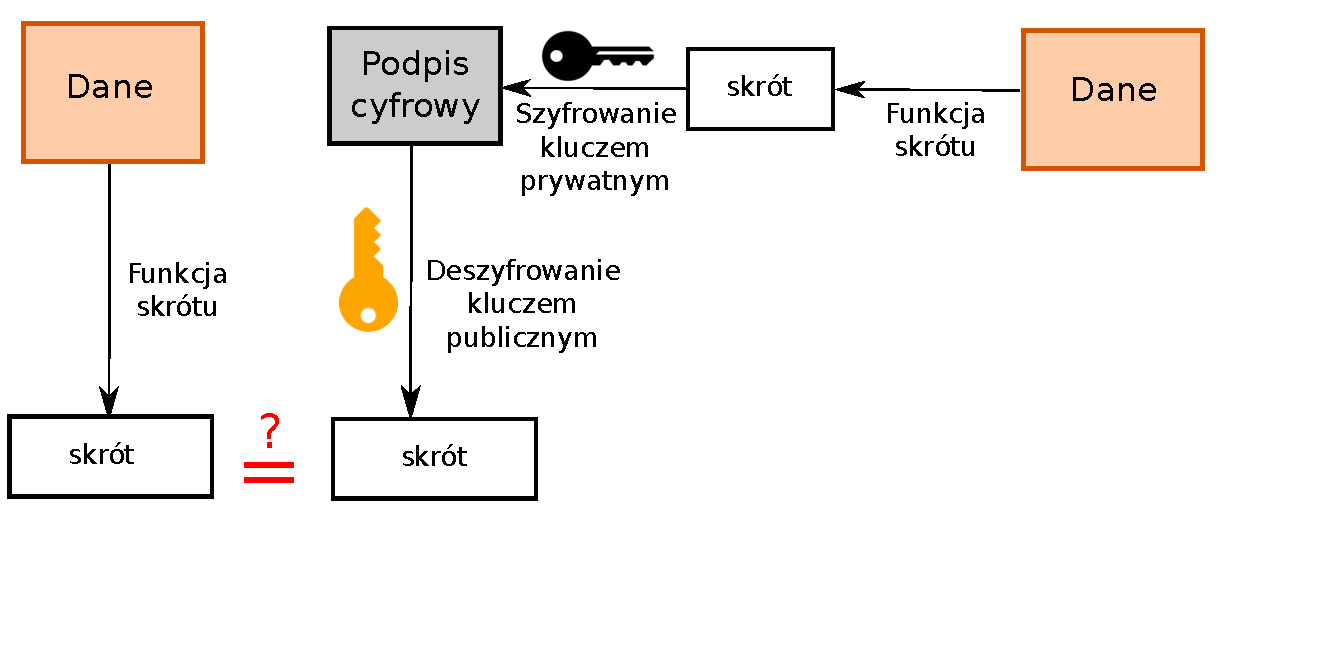
\includegraphics[height=0.5\paperwidth]{images/dig-sign.pdf}
\end{frame}
